\documentclass[12pt,a4paper]{report}
\setlength\textwidth{145mm}
 \setlength\topmargin{0mm}
 \setlength\headsep{0mm}
 \setlength\headheight{0mm}
 
% Přepneme na českou sazbu
\usepackage[czech]{babel}
\usepackage[IL2]{fontenc}
\usepackage{graphicx} 

%% Použité kódování znaků: obvykle latin2, cp1250 nebo utf8:
\usepackage[utf8]{inputenc}
\begin{document}


\section{Triviální versus Cache-oblivious implementace}
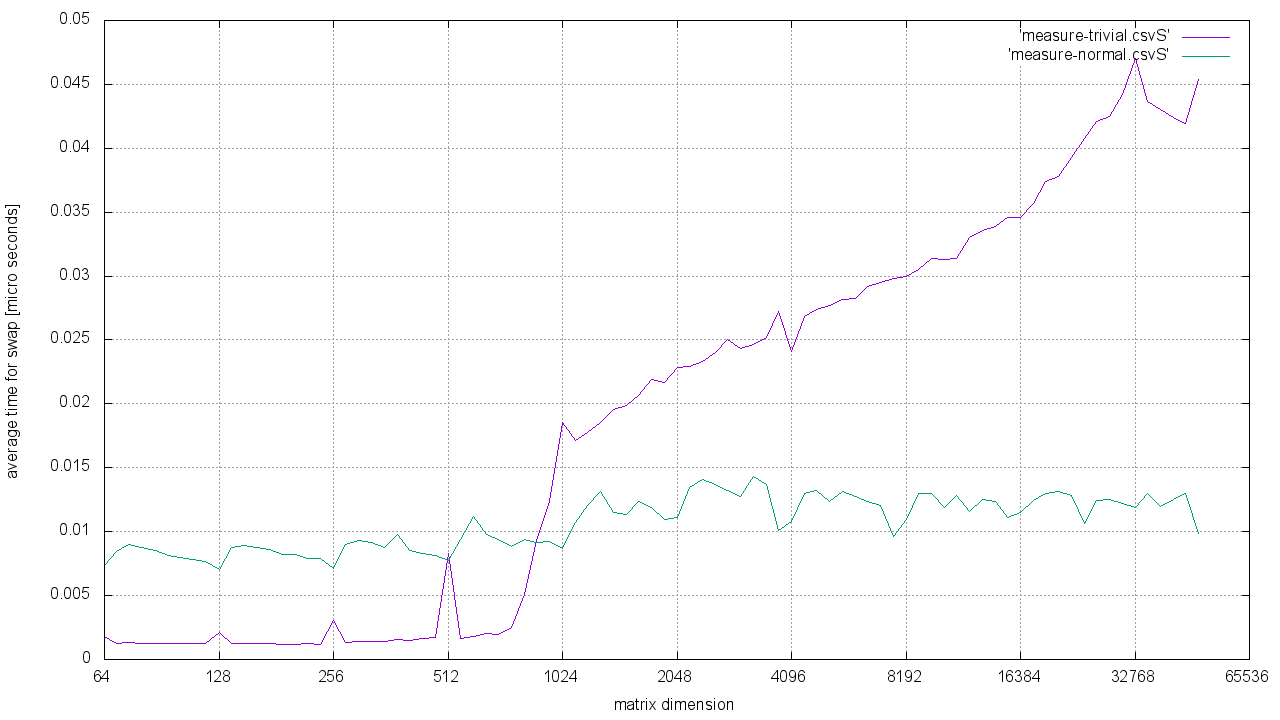
\includegraphics[width=\textwidth]{./tests/graph1.png}

Pro měření bylo použito až 10 GB paměti RAM.
Použitý počítač je osazen procesorem intel i7-920 @2.66 GHz
s 64-bitovými instrukcemi AMD64 a následujícími parametry cache:
\begin{itemize}
	\item L1 cache -- 32 kB (8 way associative - 64 B line size),
	\item L2 cache -- 256 kB (8 way associative - 64 B line size),
	\item L3 cache -- 8 MB (16 way associative - 64 B line size).
\end{itemize}

Z grafu vidíme, že zatímco průmerná doba swapu triviální implementace roste, 
tak u cache-oblivious varianty je průmerná doba swapu docela stabilní. Tipuji, že
triviální implementace je z počátku lepší, kvůli overheadu rekurze v cache-oblivious
algoritmu, navíc v triviální implementaci nedochází ještě k tolika výpadkům a do
dimenze 256 se vejde matice celá do L2 cache.
Pro dimenzi $1024$ již triviální implementace začíná nad cache-oblivious variantou
ztrácet. Pro tuto dimenzi je matice velká $4 MB$, takže se ještě celá vejde do L3 cache.

Pro cache-oblivious variantu vidíme také poklesy při velikosti dimenze přibližně $2^k$.
Jak uvidíme v další sekci, tento propad se objevuje i v simulátoru cache.

\subsection{Nárůsty na mocninách dovjky triviální verze}
Snažil jsem se odhalit příčinu těchto nárůstů a zdá se, že jsou vždy v k-násobku $512 B = 8 * 64 B$ velikosti dimenze matice
(což je velikost jedné přihrádky cache jelikož je 8 way accociative a 64 B line size).
Zkusil jsem tedy udělat podrobnější test okolo dimenze matice 384, kde by měl být $3 * 512 B$ násobek.

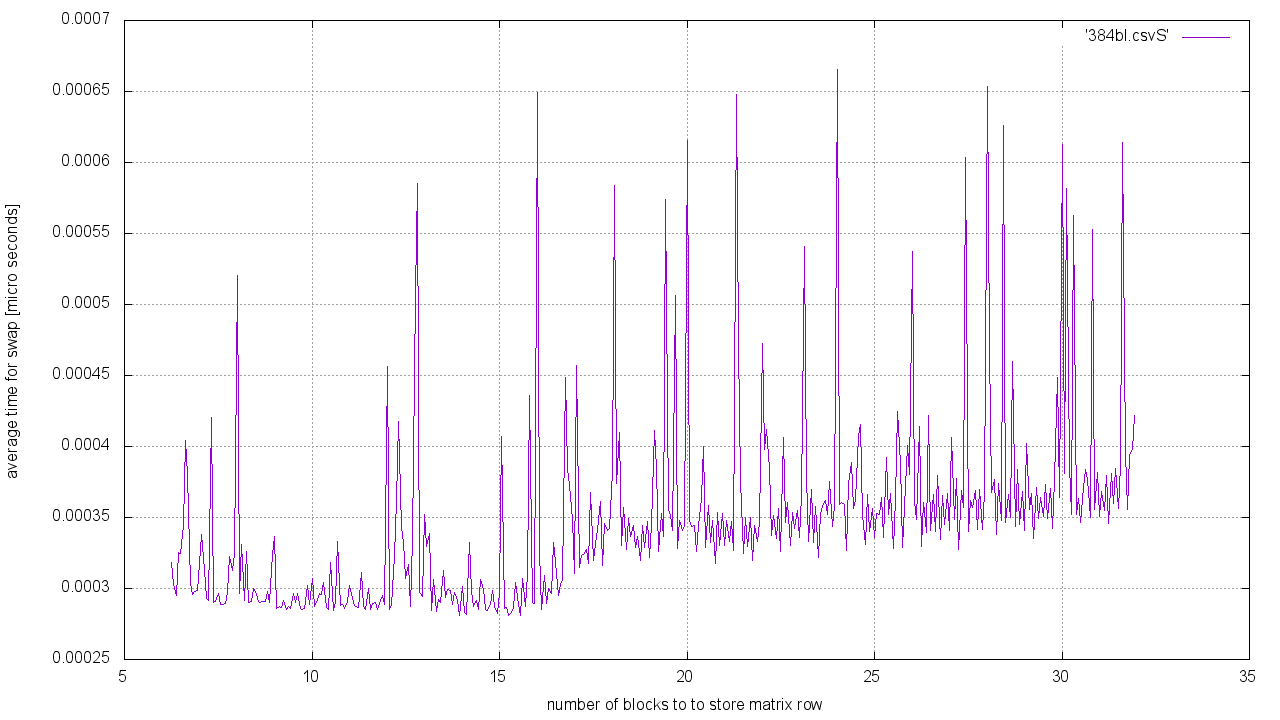
\includegraphics[width=\textwidth]{./tests/graph1-0.png}

Graf ukazuje průměrné časy na swap pro matice dimenze 100 až 511 (legenda ukazuje počet bloků, který zabírá jedna řádka matice).
Výkyvů je zde vidět mnohem více a docela pravidelně se opakují. Bližší náhled ukazuje následující graf.

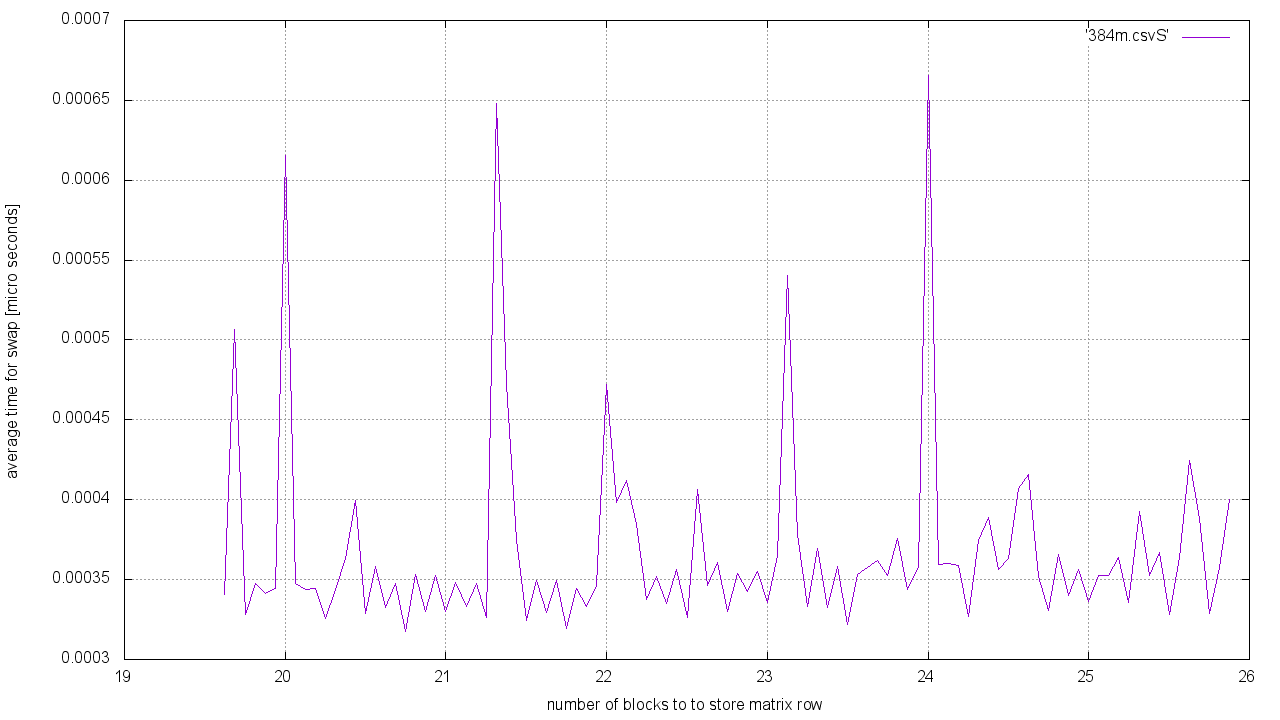
\includegraphics[width=\textwidth]{./tests/graph1-1.png}

Zdá se, že pokud má matice dimenzi přibližně rovnou násobku velikosti bloku cache ($64 B$) je na grafu navýšení. Nicméně vidíme,
zde také, že to není zcela pravidlem například pro řádky skládající se z 25 bloků.


\section{Simulace cache-oblivious algoritmu na ideální cache}
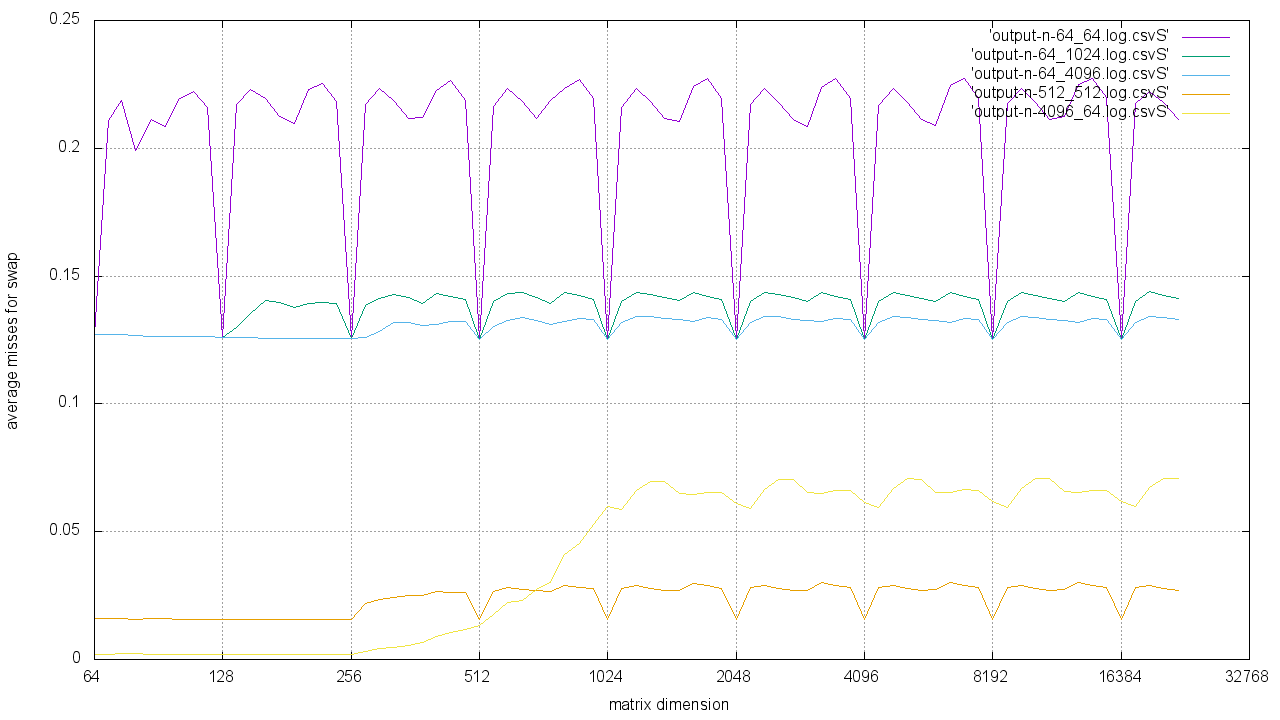
\includegraphics[width=\textwidth]{./tests/graph2.png}

Simulace jsme opět prováděli na stejných datech, jako při měření 
na počítači, nicměně pouze do maximalní velikosti matice 2 GB.
Předchozí graf znázorňuje závislost průměrného počtu missů cache na swap prvků matice cache-oblivious algoritmu.

Vidíme, že vítězem byla cache s největší kapacitou, konkrétně cache s velikostí bloku 512 B
a počtem bloků 512. Zvýšení velikosti bloků na úkor jejich počtu (4096,64) vedlo k o něco horším výsledkům pro velké matice.
Do obou těchto typu cache se vejde celá matice až po dimenzi $256$. Což vysvětluje lepší výsledky varianty (4096,64)
do zmíněného limitu.


Naopak snížení velikosti bloků ve prospěch počtu bloků (64, 4096) vedlo opět ke zvýšení průmněrného počtu missů. 
Dále už je pořadí podle celkove velikosti cache. Vidíme tak, že je třeba volit vyvážený poměr
velikosti bloků a jejich počtu, aby cache fungovala co nejlépe.

Všechny typy cache obsahují propady missů pro dimenze matice mocniny dovjky.
Řekl bych, že je to způsobeno tím, že takové matice mají všchny submatice čtvercové,
jelikož pro obdélníkové matice je třeba načíst více dat do cache, takže pro ně
bude více cache missů. Cache s menšími bloky mají propady větší, jelikož pro pro 
obdélníkové matice je třeba načíst více (a sice menších) bloků. 


\section{Simulace triviální verze algoritmu na ideální cache}
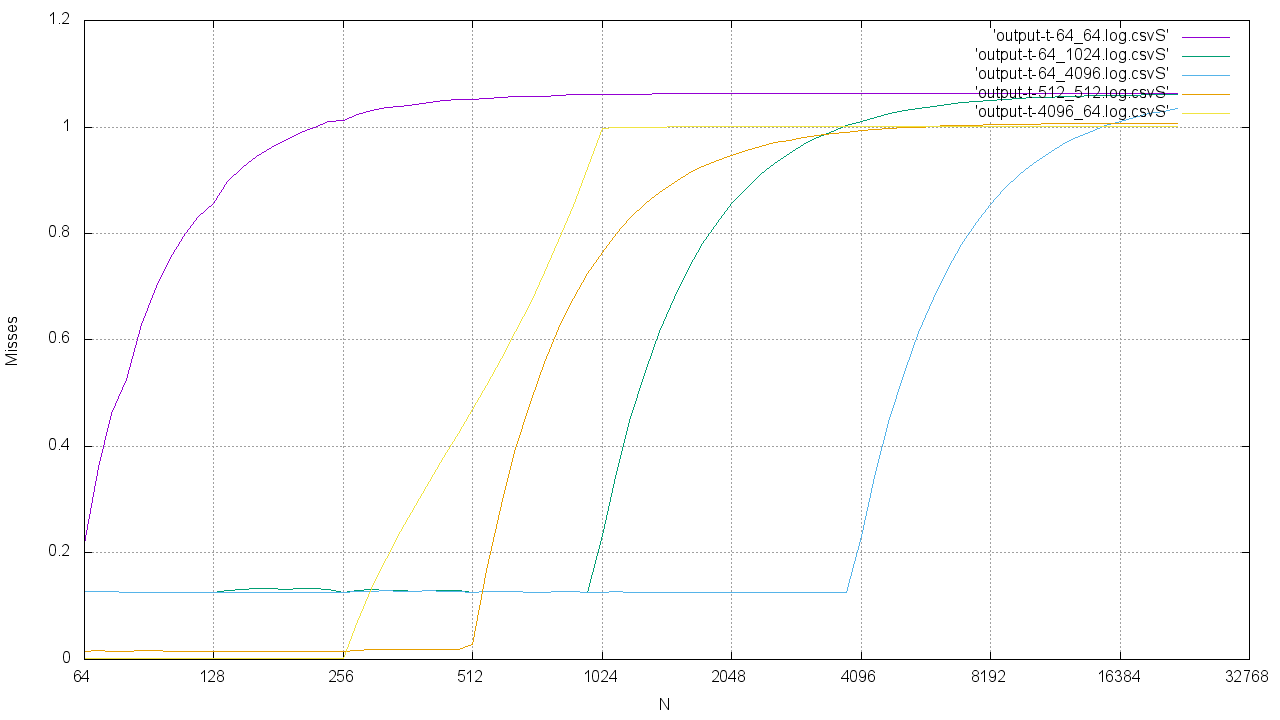
\includegraphics[width=\textwidth]{./tests/graph3.png}

Pro triviální verzi vidíme, že má řádově více cache missů. Také vidíme,
že nám nepomůže žádná verze cache, pokud velikost matice překročí velikost cache dojde 
k značnému navýšení missů.

Dále je z grafu vidět, že triviální verzi vyhovují více 
menší bloky. To je způsobeno tím, že při swapování se načítají zbytečně velké kusy řádků
matice, které nejsou potřeba (je potřeba jen jeden sloupec). Takže pro menší bloky (tudíž jejich větší počet) se může
načíst větší počet kousků řádků matice, které pak mouhou být častečně využity při swapování
dalšího řádku a sloupce. 

  
\end{document}
